\section{Расчет виртуальной энтропии и теплоемкости}
Рассчитаем виртуальную энтропию $S_{\text{вирт}}$ и теплоемкости $C_{P}$ для вещества CHCl$_3$ при температуре $T=1900$ К и давлении $P=7$ атм.

\subsection{Виртуальная энтропия}
Виртуальную энтропию можно найти как сумму поступательной, вращательной и колебательной энтропий:
\begin{equation}
S_{\text{вирт}} = S_{\text{пост}} + S_{\text{вр}} + S_{\text{кол}},
\end{equation}
где $S_{\text{пост}}$, $S_{\text{вр}}$, $S_{\text{кол}}$ --- поступательная, вращательная и колебательная энтропия соответственно.

Для начала запишем некоторые параметры молекулы
\begin{table}[h!]
	\centering
	\caption{Данные о молекуле}
	\label{tab1}
	\setlength{\extrarowheight}{1mm}
\begin{tabular}{|c|c|}
	\hline 
	\multicolumn{2}{|c|}{CHCl$_3$} \\ 
	\hline 
	Длины связей, \AA & $r_{C-H} = 1.100$ \\ 
	&	$r_{C-Cl} = 1.758$ \\
	\hline 
	Валентный угол & $\angle \text{ClCCl} = 111\degree 18'$ \\ 
	& $\angle \text{HCCl} = 107\degree 34'$ \\
	\hline 
	Частоты колебаний $\omega$, см$^{-1}$ & 3034, 680, 363, 1220 (2), 774 (2), 261 (2) \\ 
	\hline 
\end{tabular}
\end{table}
\subsubsection{Поступательная энтропия}
Поступательная энтропия для всех газообразных веществ рассчитывается по уравнению
\begin{equation}
S_{\text{пост}} = \left(\frac{3}{2}\,R\cdot \ln M+\frac{5}{2}\,R\cdot\ln T-R\cdot\ln P-9.7 \right) \cfrac{\text{Дж}}{\text{моль}\cdot\text{К}},
\end{equation}
где $M$ --- молекулярная масса в г/моль, $T$ --- температура системы в К, $P$ --- давление системы в атм.

$$
M = (12.011+1.008 + 35.453\cdot 3) \text{ г/моль} = 119.378 \text{ г/моль.}
$$

Таким образом
\begin{center}
	$S_{\text{пост}} = \left(\cfrac{3}{2} \cdot8.314\cdot \ln 119.378+\cfrac{5}{2}\cdot 8.314\cdot\ln1900-8.314\cdot\ln 7-9.7 \right) \cfrac{\text{Дж}}{\text{моль}\cdot\text{К}} = 190.68\  \cfrac{\text{Дж}}{\text{моль}\cdot\text{К}}.$
\end{center}
Итак,
\begin{equation}
\boxed{S_{\text{пост}} = 190.68\  \cfrac{\text{Дж}}{\text{моль}\cdot\text{К}}}.
\end{equation}
\subsubsection{Вращательная энтропия}
Вращательная энтропия для всех нелинейных молекул определяется по уравнению
\begin{equation}
S_{\text{вр}} = \left(\cfrac{1}{2}\,R\cdot\ln I_1I_2I_3+\cfrac{3}{2}\,R\cdot\ln T - R\cdot\ln\sigma+1320.8\right)\cfrac{\text{Дж}}{\text{моль}\cdot\text{К}},
\end{equation}
где $I_1$, $I_2$, $I_3$ --- главные значения тензора инерции многоатомной нелинейной молекулы, выражены в кг$\cdot$м$^2$, $\sigma$ --- число симметрии молекулы.

Для расчета произведения главных моментов тензора момента инерции воспользуемся методом Хиршфельдера
\begin{equation}
I_1I_2I_3 = \begin{vmatrix}
A & -D & -E\\
-D & B & -F\\
-E & -F & C\\
\end{vmatrix}
= ABC -AF^2-BE^2-CD^2-2DFE.
\end{equation}
В этой формуле
\begin{center}
	$
	A = \sum\limits_i m_i(y_i^2+z_i^2) - \cfrac{1}{\overline m}\left(\sum\limits_im_iy_i\right)^2- \cfrac{1}{\overline m}\left(\sum\limits_im_iz_i\right)^2$,\\
	$B = \sum\limits_i m_i(x_i^2+z_i^2) - \cfrac{1}{\overline m}\left(\sum\limits_im_ix_i\right)^2- \cfrac{1}{\overline m}\left(\sum\limits_im_iz_i\right)^2$,\\
	$C = \sum\limits_i m_i(x_i^2+y_i^2) - \cfrac{1}{\overline m}\left(\sum\limits_im_ix_i\right)^2- \cfrac{1}{\overline m}\left(\sum\limits_im_iy_i\right)^2$,\\
	$
	D = \sum\limits_im_ix_iy_i - \cfrac{1}{\overline m} \left(\sum\limits_im_ix_i\right)\left(\sum\limits_im_iy_i\right)$,\\	
	$
	E = \sum\limits_im_ix_iz_i - \cfrac{1}{\overline m} \left(\sum\limits_im_ix_i\right)\left(\sum\limits_im_iz_i\right)$,\\
	$
	F = \sum\limits_im_iy_iz_i - \cfrac{1}{\overline m} \left(\sum\limits_im_iy_i\right)\left(\sum\limits_im_iz_i\right)$,\\
	$\overline m = \sum\limits_i m_i$,
\end{center}
где $m_i$ --- масса, $x_i$, $y_i$, $z_i$ --- декартовы координаты i-го атома.

Расположим молекулу CHCl$_3$ так, как показано на рисунке \ref{fig:mol} (в центре -- атом углерода). 

\begin{figure}
\centering
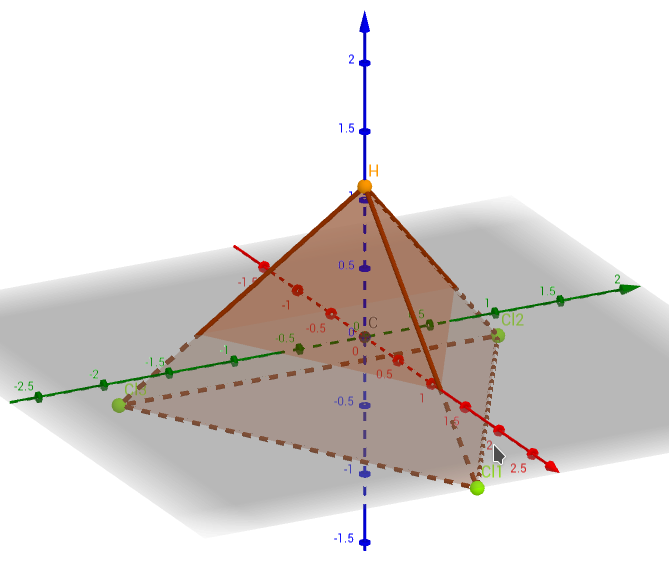
\includegraphics[width=0.7\linewidth]{mol}
\caption{}
\label{fig:mol}
\end{figure}

Тогда при выбранном начале координат и направлениях осей координаты осей будут следующими:
\begin{table}[h!]
	\centering
	\caption{Координаты атомов}
	\label{tab3}
	\setlength{\extrarowheight}{1mm}
	\begin{tabular}{|c|c|c|c|c|}
		\hline 
		Атом & $x$, \AA & $y$, \AA & $z$, \AA &  Масса атома, кг \\ 
		\hline 
		$C$ & 0 & 0 & 0 & $1.99\cdot10^{-26}$ \\ 
		\hline 
		$Cl_{(1)}$ & 1.676 & 0 & -0.530 & $5.89\cdot10^{-26}$ \\ 
		\hline 
		$Cl_{(2)}$ & -0.838 & 1.451 & -0.530 & $5.89\cdot10^{-26}$ \\ 
		\hline 
		$Cl_{(3)}$ & -0.838 & -1.451 & -0.530 & $5.89\cdot10^{-26}$ \\ 
		\hline 
		$H$ & 0 & 0 & 1.100 & $1.67\cdot10^{-27}$ \\ 
		\hline 
	\end{tabular} 
\end{table}

Найдем выражения для компонент определителя
\begin{center}
	$\overline m = \cfrac{119.378\cdot10^{-3}}{6.02\cdot10^{23}} = 1.983\cdot10^{-25}$ кг;\\
	$A = \sum\limits_i m_i(y_i^2+z_i^2) - \cfrac{1}{\overline m}\left(\sum\limits_im_iy_i\right)^2- \cfrac{1}{\overline m}\left(\sum\limits_im_iz_i\right)^2 = 2.480\cdot10^{-45} - 0 - 4.251\cdot10^{-46} = 2.055\cdot10^{-45}$ кг$\cdot$м$^2$;\\
	
	$B = \sum\limits_i m_i(x_i^2+z_i^2) - \cfrac{1}{\overline m}\left(\sum\limits_im_ix_i\right)^2- \cfrac{1}{\overline m}\left(\sum\limits_im_iz_i\right)^2 = 2.482\cdot10^{-45} - 0 - 4.251\cdot10^{-46} = 2.057\cdot10^{-45}$ кг$\cdot$м$^2$;\\
	
	$C = \sum\limits_i m_i(x_i^2+y_i^2) - \cfrac{1}{\overline m}\left(\sum\limits_im_ix_i\right)^2- \cfrac{1}{\overline m}\left(\sum\limits_im_iy_i\right)^2 =
	4.962\cdot10^{-45} - 0 - 0 = 4.962\cdot10^{-45}$ кг$\cdot$м$^2$;\\
	
	$D = \sum\limits_im_ix_iy_i - \cfrac{1}{\overline m} \left(\sum\limits_im_ix_i\right)\left(\sum\limits_im_iy_i\right) = 0 - 0 = 0$ кг$\cdot$м$^2$.
	
	$E = \sum\limits_im_ix_iz_i - \cfrac{1}{\overline m} \left(\sum\limits_im_ix_i\right)\left(\sum\limits_im_iz_i\right) = 0 - 0 = 0$ кг$\cdot$м$^2$
	
	$F = \sum\limits_im_iy_iz_i - \cfrac{1}{\overline m} \left(\sum\limits_im_iy_i\right)\left(\sum\limits_im_iz_i\right) = 0 - 0 = 0$ кг$\cdot$м$^2$
\end{center}
В итоге
$$
I_1I_2I_3 = 2.055\cdot10^{-45}\cdot2.057\cdot10^{-45}\cdot4.962\cdot10^{-45} = 2.098\cdot10^{-134}.
$$

Для данной молекулы по таблице найдем число симметрии:
$$
\sigma = 3.
$$
Таким образом
\begin{center}
	$S_{\text{вр}} = \left(\cfrac{1}{2}\,\cdot8.314\cdot\ln (2.098\cdot10^{-134})+\cfrac{3}{2}\,\cdot8.314\cdot\ln 1900 - 8.314\cdot\ln2+1320.8\right)\cfrac{\text{Дж}}{\text{моль}\cdot\text{К}}= 172.64\ \cfrac{\text{Дж}}{\text{моль}\cdot\text{К}}$
\end{center}

Итак,
\begin{equation}
\boxed{S_{\text{вр}} = 172.64\  \cfrac{\text{Дж}}{\text{моль}\cdot\text{К}}}.
\end{equation}
\subsubsection{Колебательная энтропия}
При расчете колебательной составляющей энтропии будем полагать, что молекула представлена в виде жёсткого гармонического осциллятора.

Для того, чтобы посчитать вклад $S_{i, \text{кол}}$ от каждой частоты, воспользуемся формулой
\begin{equation}
S_{i, \text{кол}} = R\,\cfrac{\frac{h\nu_i}{kT}}{e^{\frac{h\nu_i}{kT}}-1}-R\ln(1-e^{-\frac{h\nu_i}{kT}}),
\end{equation} 
или, записав ее в более удобном виде,
\begin{equation}
S_{i, \text{кол}} = R\,\cfrac{\frac{\theta_i}{T}}{e^{\frac{\theta_i}{T}}-1}-R\ln(1-e^{-\frac{\theta_i}{T}}),
\end{equation}
где $\theta_i$ --- характеристическая температура $i$-ой частоты колебаний. 

Для перевода волнового числа $\omega$ в $\theta$ надо величину $\omega$ умножить на коэффициент $\frac{ch}{k} = 1.438$, где $c$ --- скорость света, $h$ --- постоянная Планка, $k$ --- постоянная Больцмана.

Составим для удобства расчетов таблицу.
\begin{table}[h!]
	\centering
	\caption{Колебательная энтропия}
	\label{tab2}
	\setlength{\extrarowheight}{1mm}
	\begin{tabular}{|c|c|c|c|}
		\hline
		$\omega$, см$^{-1}$ & $\theta$, К & $\frac{\theta}{T}$ & $S_{i,\text{кол}}$, $\frac{\text{Дж}}{\text{моль}\cdot\text{К}}$ \\
		\hline 
		3034 & 4363 & 2.30 & 3.01 \\ 
		\hline 
		680 & 978 & 0.51 & 14.00 \\ 
		\hline 
		363 & 522 & 0.27 & 19.23 \\ 
		\hline 
		1220 (2) & 1754 & 0.92 & 9.29 \\ 
		\hline 
		774 (2) & 1113 & 0.59 & 12.82 \\ 
		\hline 
		261 (2) & 375 & 0.20 & 21.71 \\ 
		\hline 
		\multicolumn{3}{|c|}{} & $\sum\limits_i S_{i,\text{кол}} = 80.06$ \\ 
		\hline 
		\end{tabular} 
\end{table}

Итак,
\begin{equation}
\boxed{S_{\text{кол}} = 80.06\  \cfrac{\text{Дж}}{\text{моль}\cdot\text{К}}}.
\end{equation}
\subsubsection{Окончательное значение виртуальной энтропии}
Таким образом, виртуальная энтропия CHCl$_3$ равна
\begin{center}
$S_{\text{вирт}} = S_{\text{пост}} + S_{\text{вр}} + S_{\text{кол}} = 190.68+172.64+80.06 = 443.38\ \cfrac{\text{Дж}}{\text{моль}\cdot\text{К}}$
\end{center}
Итоговый результат
\begin{equation}
\boxed{S_{\text{вирт}} = 443.38\  \cfrac{\text{Дж}}{\text{моль}\cdot\text{К}}}.
\end{equation}

\subsection{Теплоемкость $C_P$}
Теплоемкость $C_P$ можно найти как сумму поступательной, вращательной и колебательной теплоемкостей
\begin{equation}
C_P = C_{\text{пост}} + C_{\text{вр}} + C_{\text{кол}},
\end{equation}
где $C_{\text{пост}}$, $C_{\text{вр}}$, $C_{\text{кол}}$ --- поступательная, вращательная и колебательная теплоемкость соответственно.

Найти $C_{\text{пост}}$ и $C_{\text{вр}}$ не составляет труда (молекула CHCl$_3$ не является линейной)
\begin{equation}
C_{\text{пост}} = \cfrac{5}{2}\,R \qquad C_{\text{вр}} = \cfrac{3}{2}\,R.
\end{equation}

Для расчета колебательной теплоемкости воспользуемся формулой
\begin{equation}
C_{i,\text{кол}} =R\, \cfrac{\left(\frac{\theta_i}{T}\right)^2e^{\frac{\theta_i}{T}}}{\left(e^{\frac{\theta_i}{T}}-1\right)^2}.
\end{equation}

Составим для удобства расчетов таблицу.

\begin{table}[h!]
	\centering
	\caption{Колебательная теплоемкость}
	\label{tab2}
	\setlength{\extrarowheight}{1mm}
	\begin{tabular}{|c|c|c|c|}
		\hline
		$\omega$, см$^{-1}$ & $\theta$, К & $\frac{\theta}{T}$ & $C_{i,\text{кол}}$, $\frac{\text{Дж}}{\text{моль}\cdot\text{К}}$ \\
		\hline 
		3034 & 4363 & 2.30 & 5.45 \\ 
		\hline 
		680 & 978 & 0.51 & 8.14 \\ 
		\hline 
		363 & 522 & 0.27 & 8.26 \\ 
		\hline 
		1220 (2) & 1754 & 0.92 & 7.75 \\ 
		\hline 
		774 (2) & 1113 & 0.59 & 8.08 \\ 
		\hline 
		261 (2) & 375 & 0.20 & 8.29 \\ 
		\hline 
		\multicolumn{3}{|c|}{} & $\sum\limits_i C_{i,\text{кол}} = 45.97$ \\ 
		\hline 
	\end{tabular} 
\end{table}
\vspace{5cm}
Таким образом
$$
C_P = C_{\text{пост}} + C_{\text{вр}} + C_{\text{кол}} = \cfrac{5}{2}\,8.314 + \cfrac{3}{2}\,8.314+45.97 = 79.27\ \frac{\text{Дж}}{\text{моль}\cdot\text{К}}
$$

Итоговый результат
\begin{equation}
\boxed{C_P = 79.27\  \cfrac{\text{Дж}}{\text{моль}\cdot\text{К}}}.
\end{equation}

\subsection{Сопоставим результат с уравнением энтропии}
Сопоставим результаты расчета с уравнением
\begin{equation}
S = S_{298}^0 + \int\limits_{298}^{1900}\cfrac{C_P(T) dT}{T}-R\ln P,
\end{equation}
где $C_P(T) = C_{\text{пост}} + C_{\text{вр}} + C_{\text{кол}}(T)$, $S_{298}^0 = 296.48\ \frac{\text{Дж}}{\text{моль}\cdot\text{К}}$ (табличная величина). 

Подставив все значения, получим
\begin{multline}
S = 296.48  + \\ + 8.314\,\cdot \int\limits_{298}^{1900}\left(\frac{(4363/T)^2\cdot e^{\frac{4363}{T}}}{(e^{\frac{4363}{T}}-1)^2} + \frac{(978/T)^2\cdot e^{\frac{978}{T}}}{(e^{\frac{978}{T}}-1)^2} + \frac{(522/T)^2\cdot e^{\frac{522}{T}}}{(e^{\frac{522}{T}}-1)^2} + 2\cdot\frac{(1754/T)^2\cdot e^{\frac{1754}{T}}}{(e^{\frac{1754}{T}}-1)^2} +\right. \\ \left. + 2\cdot\frac{(1113/T)^2\cdot e^{\frac{1113}{T}}}{(e^{\frac{1113}{T}}-1)^2} + 2\cdot\frac{(375/T)^2\cdot e^{\frac{375}{T}}}{(e^{\frac{375}{T}}-1)^2} + 4\right)\cdot\cfrac{dT}{T}  -8.314\cdot\ln7 = 443.74 \ \cfrac{\text{Дж}}{\text{моль}\cdot\text{К}}
\end{multline}

Итак,
\begin{equation}
\boxed{S = 443.74 \ \cfrac{\text{Дж}}{\text{моль}\cdot\text{К}}}.
\end{equation}

Величины сходятся.

\subsection{Температура равенства вращательной и колебательной энтропий}
Для того, чтобы найти температуру, при которой вращательная и колебательная энтропии станут равны, составим уравнение и разрешим его относительно температуры
\begin{equation}
\cfrac{1}{2}\,R\cdot\ln I_1I_2I_3+\cfrac{3}{2}\,R\cdot\ln T - R\cdot\ln\sigma+1320.8 = \sum\limits_{i=1}^6 g\left[ R\,\cfrac{\frac{\theta_i}{T}}{e^{\frac{\theta_i}{T}}-1}-R\ln(1-e^{-\frac{\theta_i}{T}})\right]
\end{equation}
где $g$ -- степень вырождения уровня.

Используя ЭВМ, получим значение
$$
\boxed{T_{\text{энтр}} = 1612 \text{ К}}
$$

\subsection{Температура равенства вращательной и колебательной теплоемкостей}
Для того, чтобы найти температуру, при которой вращательная и колебательная теплоемкости станут равны, составим уравнение и разрешим его относительно температуры
\begin{equation}
\sum\limits_{i=1}^6 R\, \cfrac{\left(\frac{\theta_i}{T}\right)^2e^{\frac{\theta_i}{T}}}{\left(e^{\frac{\theta_i}{T}}-1\right)^2} = \cfrac{3}{2}\,R
\end{equation}
Используя ЭВМ, получим значение
$$
\boxed{T_{\text{тепл}} = 135.5 \text{ К}}
$$
\subsection{Аппроксимационное уравнение $C_P(T)$}	
Мы нашли зависимость $C_P(T)$
\begin{equation}
C_P(T) = C_{\text{пост}} + C_{\text{вр}} + \sum\limits_{i=1}^6 R\, \cfrac{\left(\frac{\theta_i}{T}\right)^2e^{\frac{\theta_i}{T}}}{\left(e^{\frac{\theta_i}{T}}-1\right)^2}
\end{equation}

С помощью Python можно аппроксимировать данное уравнение полиномом третьей степени в пределах температур от 298 К до 1000 К:
\begin{equation}
C_P(T) = 24.394 + 1.859\cdot10^{-1} T  - 1.794\cdot10^{-4}T^2 + 6.483\cdot10^{-8}T^3
\end{equation}

Отобразим зависимость на графике
\begin{figure}[h!]
	\centering
	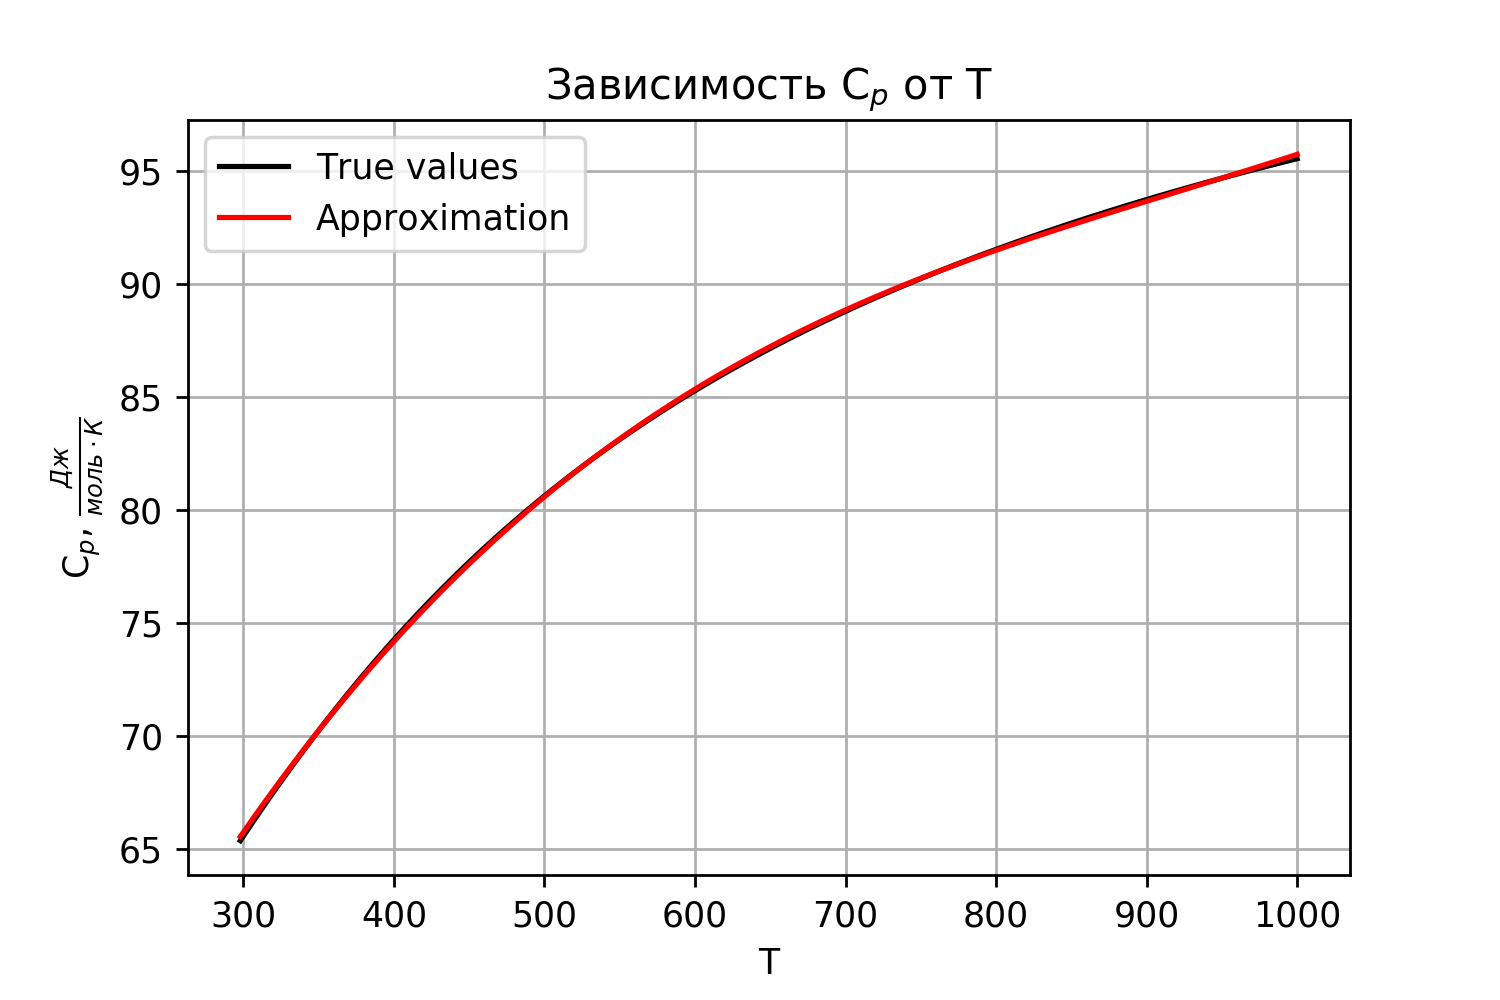
\includegraphics[width=0.88\linewidth]{approx}
	\caption{Зависимость $C_P(T)$}
	\label{fig:approximate}
\end{figure}

Аппроксимация полиномом 3-ей степени отлично описывает нашу зависимость.


\bibliography{mybibliography}
\bibliographystyle{gost705}